\chapter{Redes Definidas por Software}

\section{Definição Geral} As Redes Definidas
por Software (\textit{Software Defined Networks}, ou \textit{SDN}) constituem
um novo paradigma para o desenvolvimento de pesquisas em
redes de computadores que vem ganhando a atenção de grande
parte da comunidade acadêmica e da industria da área de
redes. Fazendo um balanço geral da situação que encontramos
hoje, podemos dizer que é um pouco complexa: é possível afirmar
que a área de redes fez um sucesso estrondoso, já que hoje a
tecnologia de redes de computadores permeia todos os níveis
da sociedade. Grande parte das atividades da sociedade de
alguma forma passa por uma ou mais redes de computadores.

Mas tamanho sucesso trouxe consigo um problema para a comunidade
de pesquisa. Como grande parte da sociedade depende hoje da
Internet em suas atividades diárias e as tecnologias de rede
se tornaram de fácil acesso, a estabilidade se tornou uma
característica fundamental das redes de computadores. Isso
significa que pesquisas com novas tecnologias e protocolos
já não são mais possíveis em redes de larga escala, como a
Internet, devido ao risco de interrupção ou instabilidade
dos serviços essenciais. Outro problema encontrado pelos
pesquisadores é o fato de que a larga utilização de
tecnologias já desenvolvidas inviabiliza a inserção de
qualquer tecnologia que exija a inserção de novos
equipamentos de hardware.

Mesmo pesquisadores trabalhando em redes experimentais sofrem
para justificar a adoção em larga escala das tecnologias
desenvolvidas nesses ambientes. O potencial de instabilidade
ou ruptura de tais avanços se torna um forte argumento
contra sua adoção.

Esses problemas citados acima só ocorrem pelo fato de que redes
de computadores em geral e a rede mundial (a Internet)
atingiram um nível de amadurecimento que as tornaram pouco 
flexíveis.
Para tentar melhorar essa situação, a comunidade de pesquisa
em redes de computadores tem investido em iniciativas que
levam ao desenvolvimento de redes com maiores 
recursos de programação, de forma que as novas tecnologias
possam ser inseridas na rede de forma gradual. Exemplos de
iniciativas desse tipo são as propostas de redes ativas
\textit{(active networks)} [Tennenhouse e Wetherall 2007],
de \textit{testbeds} como o PlanetLab [Peterson e Roscoe 2006]
e, mais recentemente, do GENI [Turner 2006, Elliott e Falk
2009]. Redes ativas, apesar de terem grande potencial,
tiveram pouca aceitação pela necessidade de alteração dos
elementos de rede para permitir que se tornassem programáveis. As iniciativas 
mais recentes, como o PlanetLab e o GENI, apostam na adoção
de recursos de virtualização para facilitar a transição para
novas tecnologias. Apesar de serem consideradas de
grande potencial ao longo prazo, tais iniciativas ainda
enfrentam desafios em questões como garantir o desempenho
exigido pelas aplicações largamente utilizadas hoje
utilizando-se tais elementos de rede virtualizados.

Uma outra forma de abordar o problema, a fim de oferecer
um caminho de menor impacto e que possa ser implementado 
em prazos mais curtos e com bom desempenho, consiste
em estender o hardware de encaminhamento de pacotes
de forma mais restrita. Considerando-se que a operação 
que precisa de alto desempenho nos elementos de comutação
atual é o encaminhamento de pacotes, algumas iniciativas
propõem manter essa operação pouco alterada, para manter 
a viabilidade de desenvolvimento de hardware de alto
desempenho, mas com uma possibilidade de maior controle 
por parte dos administradores de rede. Essa proposta se inspira 
em uma tecnologia já largamente adotada, o chaveamento
(encaminhamento) baseado em rótulos programáveis, 
popularizado pelo MPLS \textit{(Multi-Protocol Label
 Switching)} [Davie e Farrel 2008, Kempf et al. 2001].

Com o MPLS, o controle fino sobre o tráfego de rede se torna 
possível ao se atribuir a cada pacote um rótulo \textit{(label)}
que determina como o mesmo será tratado pelos elementos
de rede. Explorando esse recurso, administradores de rede podem
exercer controle diferenciado sobre cada tipo de tráfego de rede,
assumindo que os mesmos possam ser identificados para
receberem os rótulos apropriados. Com base nessa observação,
uma ideia trabalhada por diversos pesquisadores é a manutenção 
de um hardware de encaminhamento de alto desempenho, com
a possibilidade de permitir que os administradores de redes (ou 
os desenvolvedores de aplicações para a rede) determinem como 
os fluxos irão ser rotulados e encaminhados.

A iniciativa mais bem sucedida nesse sentido foi, sem dúvida,
definição da interface e do protocolo OpenFlow [McKeown et al.
2008]. Com o OpenFlow, os elementos de encaminhamento 
oferecem uma interface de programação simples que lhes
permite estender o acesso e controle da tabela de consulta 
utilizada pelo hardware para determinar o próximo passo de 
cada pacote recebido. Dessa forma, o encaminhamento continua 
sendo eficiente, pois a consulta à tabela de encaminhamento 
continua sendo tarefa do hardware, mas a decisão sobre 
como cada pacote deve ser processado pode ser transferida
para um nível superior, onde diferentes funcionalidades 
podem ser implementadas. Essa estrutura permite que a rede
seja controlada de forma extensível através de aplicações,
expressas em software. A esse novo paradigma, deu-se o 
nome de Redes Definidas por Software, ou \textit{Software
Defined Networks} (SDN).

Do ponto de vista histórico, as Redes Definidas por 
Software têm sua origem na definição
da arquitetura de redes \textit{Ethane}, que definia uma forma
de se implementar políticas de controle de acesso de forma 
distribuída, a partir de um mecanismo de supervisão centralizado
[Casado et al. 2009]. Naquela arquitetura, cada elemento de 
rede deveria consultar o elemento supervisor ao identificar um
novo fluxo. O supervisor consultaria um grupo de políticas 
globais para decidir, com base nas características de cada
fluxo, como o elemento de encaminhamento deveria 
tratá-lo. Essa decisão seria comunicada ao comutador na 
forma de programação de uma entrada em sua tabela de
encaminhamento com uma regra adequada para o novo fluxo (
que poderia, inclusive, ser seu descarte). Esse modelo foi
posteriormente formalizado por alguns autores na forma da 
arquitetura \textit{OpenFlow}.

\section{Introdução ao Protocolo \textit{OpenFlow}}

O \textit{OpenFlow} foi proposto pela Universidade de
Stanford para atender à demanda de validação de novas
propostas de arquiteturas e protocolos de rede (incluindo as
abordagens \textit{clean slate}) sobre equipamentos
comerciais. É definido como uma padrão aberto para Redes
Definidas por Software que tem como principal objetivo que 
se utilize equipamentos comerciais para pesquisa e 
experimentação de novos protocolos de rede, em paralelo
com a operação normal das redes. Isso é conseguido com a 
definição de uma interface de programação que permite 
ao desenvolvedor controlar diretamente os elementos de 
encaminhamento de pacotes presentes no dispositivo. Com o 
\textit{OpenFlow}, pesquisadores podem utilizar equipamentos de 
rede comerciais, que normalmente possuem maior poder 
de processamento que os comutadores utilizados em 
laboratórios de pesquisa, para realizar experimentos em redes
"de produção". Isso facilita muito a transferência dos resultados
de pesquisa para a indústria. 

\section{Descrição Geral do Protocolo \textit{OpenFlow}}

Uma característica básica da arquitetura do padrão \textit{OpenFlow} 
é a separação clara entre os planos de dados e controle em
elementos de chaveamento. O plano de dados cuida do 
encaminhamento de pacotes com base em regras simples (chamadas de ações 
na terminologia \textit{OpenFlow}) associadas
a cada entrada da tabela de encaminhamento do comutador 
de pacotes (podendo ser um \textit{switch}, um roteador 
ou até mesmo um ponto de acesso sem fio).
Essas regras, definidas pelo padrão, incluem (\textit{i}) 
encaminhar o pacote para uma porta específica do dispositivo,
(\textit{ii}) alterar parte de seus cabeçalhos, (\textit{iii}) 
descartá-los, ou (\textit{iv}) encaminhá-lo para inspeção 
por um controlador da rede. Em dispositivos dedicados, o plano
de dados pode ser implementado em hardware utilizando os
elementos comuns aos roteadores e \textit{switches} atuais.
Já o módulo de controle (ou controlador) pode ser um 
módulo de software implementado de forma independente em
algum ponto da rede.

A principal abstração utilizada na especificação
\textit{OpenFlow} é o conceito
de fluxo. Um fluxo é constituído pela combinação de campos
do cabeçalho do pacote a ser processado pelo dispositivo,
conforme Figura \ref{fig:cabecalhoOpenflow}. As tuplas podem
ser formadas por campos das camadas de enlace, de rede ou de
transporte, segundo o modelo \textit{TCP/IP}. Deve-se
enfatizar que a abstração da tabela de fluxos ainda está sujeita a
refinamentos, com o objetivo de oferecer uma melhor
exposição dos recursos do hardware e, nesse caso, permitir a
concatenação de várias tabelas já disponíveis, como, por
exemplo, tabelas \textit{IP/Ethernet/MPLS}. Nesse sentido, a
contribuição mais importante do paradigma do
\textit{OpenFlow} é a generalização do plano
de dados – qualquer modelo de encaminhamento de dados
baseado na tomada de decisão fundamentada em algum valor, ou
combinação de valores, dos campos de cabeçalho dos pacotes
pode ser suportado.

\begin{figure}[hb] \centering
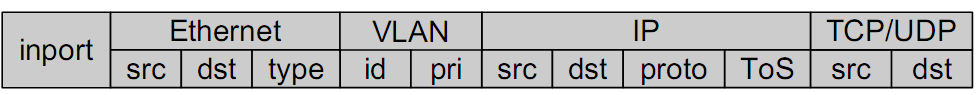
\includegraphics[width=160mm]{cabecalhoOpenflow.png}
\caption{Cabeçalho \textit{OpenFlow} para a especificação dos fluxos}
\label{fig:cabecalhoOpenflow}
\end{figure}

Um grande trunfo da arquitetura \textit{OpenFlow} é a flexibilidade 
que ela oferece para se programar de forma independente do
tratamento de cada fluxo observado, do ponto de vista de como
o mesmo deve (ou não) ser encaminhado pela rede. Basicamente,
o padrão \textit{OpenFlow} determina como um fluxo pode ser definido,
as ações que podem ser realizadas para cada pacote pertencente
a um fluxo e o protocolo de comunicação entre o comutador de 
pacotes e o controlador, utilizado para realizar alterações dessas 
definições e ações. A união de uma definição de fluxo e um
conjunto de ações forma uma entrada da tabela de fluxos 
\textit{OpenFlow} [McKeown et al. 2008].

Em um \textit{switch} \textit{OpenFlow}, cada entrada na tabela de 
fluxos pode ser implementada como um padrão de bits 
representado em uma memória TCAM (\textit{Ternary Content-
Addressable Memory}). Nesse tipo de memória, bits podem
ser representados como zero, um ou "não importa" 
(\textit{don't care}), indicando que ambos os valores são
aceitáveis naquela posição. Como o padrão é programado
a partir do plano de controle, fluxos podem ser definidos da 
forma escolhida pelo controlador. A Figura \ref{fig:fluxoopenflow}
apresenta uma visão geral de uma entrada da tabela \textit{OpenFlow}.
Cada pacote que chega a um comutador \textit{OpenFlow} é comparado
com cada entrada dessa tabela; caso um casamento seja encontrado,
considera-se que o pacote pertence àquele fluxo e aplica-se
as ações relacionadas à esse fluxo. Caso um casamento não
seja encontrado, o pacote é encaminhado para o controlador 
para ser processado -- o que pode resultar na criação de uma
nova entrada para aquele fluxo. Além das ações, a arquitetura
prevê a manutenção de três contadores por fluxo: pacotes,
 \textit{bytes} trafegados e duração do fluxo. Esses contadores são 
implementados para cada entrada da tabela de fluxos e 
podem ser acessados pelo controlador através do protocolo
\textit{OpenFlow}.

\begin{figure}[hb] \centering
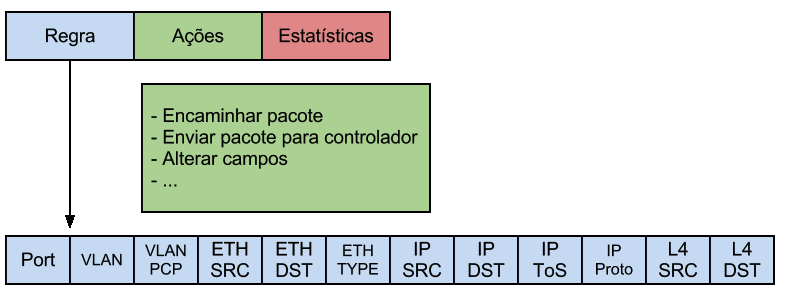
\includegraphics[width=160mm]{fluxoOpenflow.png} 
\caption{Exemplo de uma entrada na tabela de fluxos \textit{OpenFlow}.} 
\label{fig:fluxoopenflow} 
\end{figure}

Esse pequeno conjunto de regras cria diversas possibilidades,
pois muitas das funcionalidades que são implementadas 
separadamente podem ser agrupadas em um único controlador
\textit{OpenFlow}, utilizando um pequeno conjunto de regras. Alguns 
exemplos das possibilidades são apresentados na Figura \ref{fig:exemploSwitchOpenFlow}.
As entradas representam o uso do \textit{switch} \textit{OpenFlow}
para realizar encaminhamento de pacotes na camada de enlace,
implementar um firewall e realizar encaminhamento de pacotes 
na camada de enlace utilizando redes virtuais (VLANs), respectivamente.

\begin{figure}[h] \centering
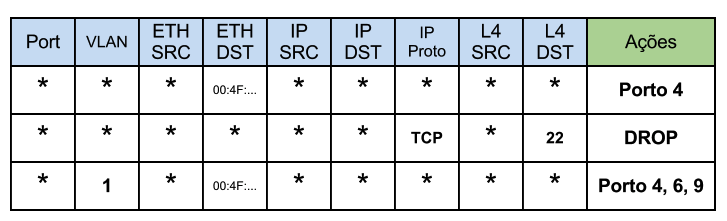
\includegraphics[width=160mm]{exemploSwitchOpenFlow.png} 
\caption{Exemplos de uso de um \textit{switch OpenFlow}.} 
\label{fig:exemploSwitchOpenFlow} 
\end{figure}

Apesar de possuir um conjunto pequeno de ações simples, 
alguns pesquisadores descrevem o \textit{OpenFlow} como uma analogia ao conjunto 
de instruções de um microprocessador x86 que, apesar de 
pequeno e simples, provê uma vasta gama de possibilidades 
para o desenvolvimento de aplicações. O \textit{OpenFlow} cria 
possibilidades semelhantes para o desenvolvimento de 
aplicações no contexto de redes de computadores. 

A versão atual do \textit{OpenFlow} ainda possui algumas limitações
em termos do uso padrão em circuitos ópticos e uma definição 
de fluxos que englobe protocolos que não fazem parte do 
modelo TCP/IP. No entanto, está sendo formulada uma nova
versão cujo objetivo é eliminar algumas dessas limitações.

A Figura \ref{fig:openflow} define de forma introdutória uma 
rede de computadores com o protocolo \textit{OpenFlow} habilitado. Os 
elementos comutadores podem ser de qualquer tipo, como 
comutadores convencionais, roteadores ou até mesmo pontos
de acesso sem fio. Podemos ver o elemento externo, chamado
de controlador, tomando contas das regras e ações instaladas
no hardware de rede. O controlador pode ser executado em 
qualquer equipamento com suporte a redes, como um 
servidor comum.

\begin{figure}[h] \centering
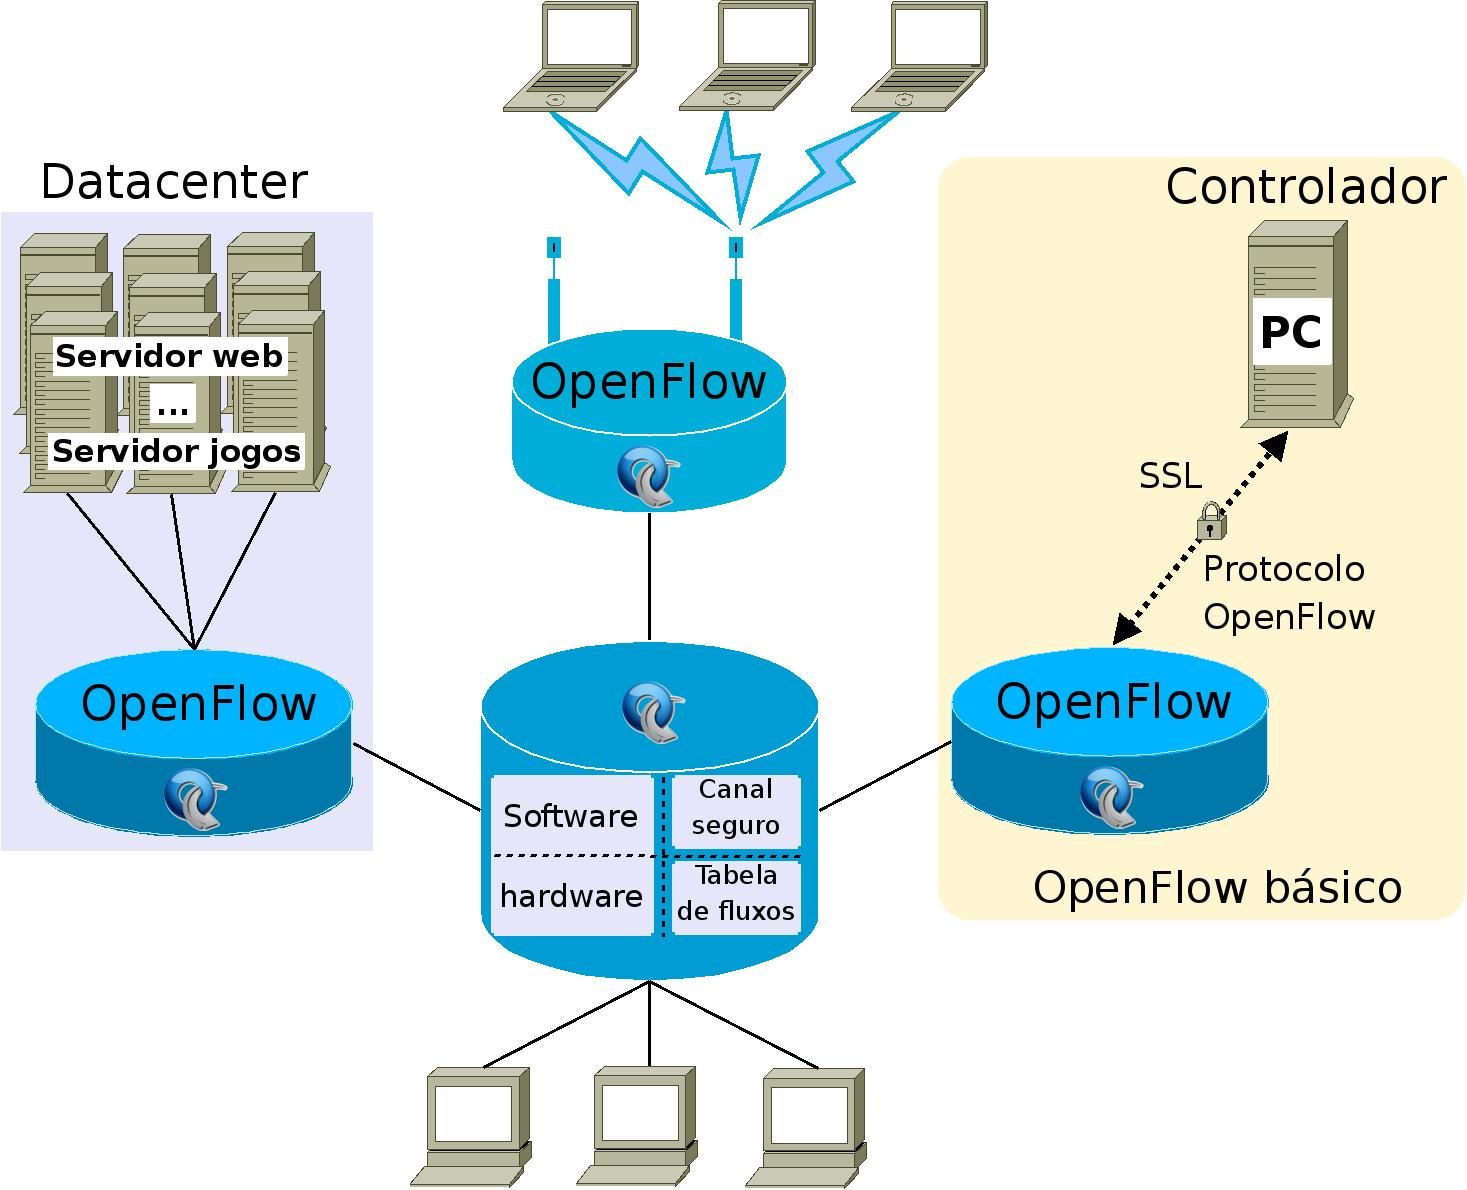
\includegraphics[width=130mm]{openflow.png} 
\caption{Rede com o protocolo \textit{OpenFlow} habilitado.} 
\label{fig:openflow} 
\end{figure}